\bframe{KL}
\begin{center}
  Masses are $p$, center of mass: \\
  $\sum p q/p  = \sum q = 1$, $KL = \sum p \log q/p >= 0$
  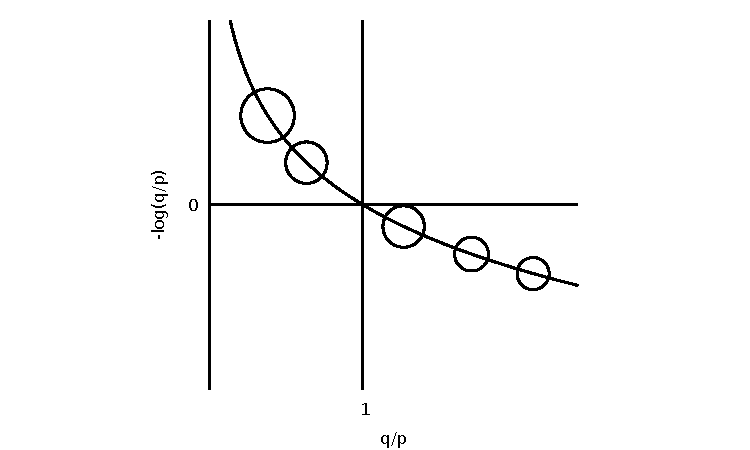
\includegraphics[width=\textwidth]{i/kl.pdf}
\end{center}
\eframe

\bframe{KL}

In population $p_1 + p_2 = 1$. Prob. of a sample $n_1 + n_2 = N$ is
\begin{equation*}
P \propto p_1^{n_1} p_2^{n_2} \propto p_1^{q_1} p_2^{q_2}
\end{equation*}
where $q = n / N$
\begin{equation*}
\log P = \sum q \log p
\end{equation*}
A maximum of $P$ is for $q = p$.
\begin{equation*}
KL = \sum p \log p - \sum q \log p
\end{equation*}
\eframe

\bframe{Clustering}
$x$ -- coordinates data, $\theta$ --- parameters of two normal distributions, $z$ --- "color" configuration
\begin{center}
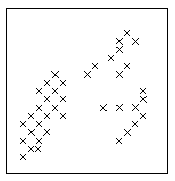
\includegraphics[width=0.6\textwidth]{i/km.pdf}
\end{center}
\eframe

\bframe{Clustering}
\begin{center}
\includegraphics[width=0.8\textwidth]{i/soft.pdf}
\end{center}
\eframe

\bframe{EM}

Distributions $p(x) = m$, $p(x, z) = j$, $p(z | x) = c$, $\sum q = 1$, $\sum c = 1$, $q = q_+ q_- $

\begin{equation*}
m = \frac{j}{c} = \frac{j/q}{c/q}
\end{equation*}

\begin{equation*}
\log m = \log \frac{j}{q} - \log \frac{c}{q}
\end{equation*}

\begin{equation*}
\log m = \sum q \log \frac{j}{q} - \sum q \log \frac{c}{q} = L(q, j) + KL(q, c)
\end{equation*}

\eframe

\bframe{Var}
\begin{equation*}
L(q, j) = \sum_+ q_+  \sum_-  q_- \log j -  \sum_+ q_+  \log q_+
\end{equation*}

\begin{equation*}
\log q_+^* = \sum_- q_- \log j   + const
\end{equation*}

\begin{equation*}
q_+^* = \frac{ \exp( \sum_- q_- \log j)}{    \sum_+  \exp(\sum_- q_ - \log j) }
\end{equation*}

\begin{equation*}
q_- = \delta(z_- - \theta)
\end{equation*}

\begin{equation*}
q_+^* = \frac{ j(\theta, z_+)}{  \sum_+ j(\theta, z_+) } = c
\end{equation*}
\eframe

\bframe{VI}
\begin{center}
\includegraphics[width=0.8\textwidth]{i/sigma.pdf}
\end{center}

\eframe


